\subsection{DNR with CRF}

The second implementation trains a Conditional Random Fields model to perform classification of BIO tag for each word as a means of Drug Name Recognition. All code is based on Python 3 and Scikit-learn and sklearn-crfsuite. As before it uses modules for interacting with Freeling, perform the lookup of words on a DrugBank lookup and the like. This time, the model feature matrix input will be the sequence of features for each word of a sentence. 

\textbf{Features}

The complete set of features prepared for this model is the same used in the previous smv model \ref{table:DNRfeatures}.

\textbf{Feature vector}

The CRF model is trained on a sequence of word features basis. This includes all the possible features of a word and the words in a context window of 0 to 5, concatenated in a sequence for each sentence in the training data set. The structure of the feature vector for each word is shown in the figure \ref{dnrcrf}.


\begin{figure}[H]
\minipage{0.5\textwidth}%
  \centering
  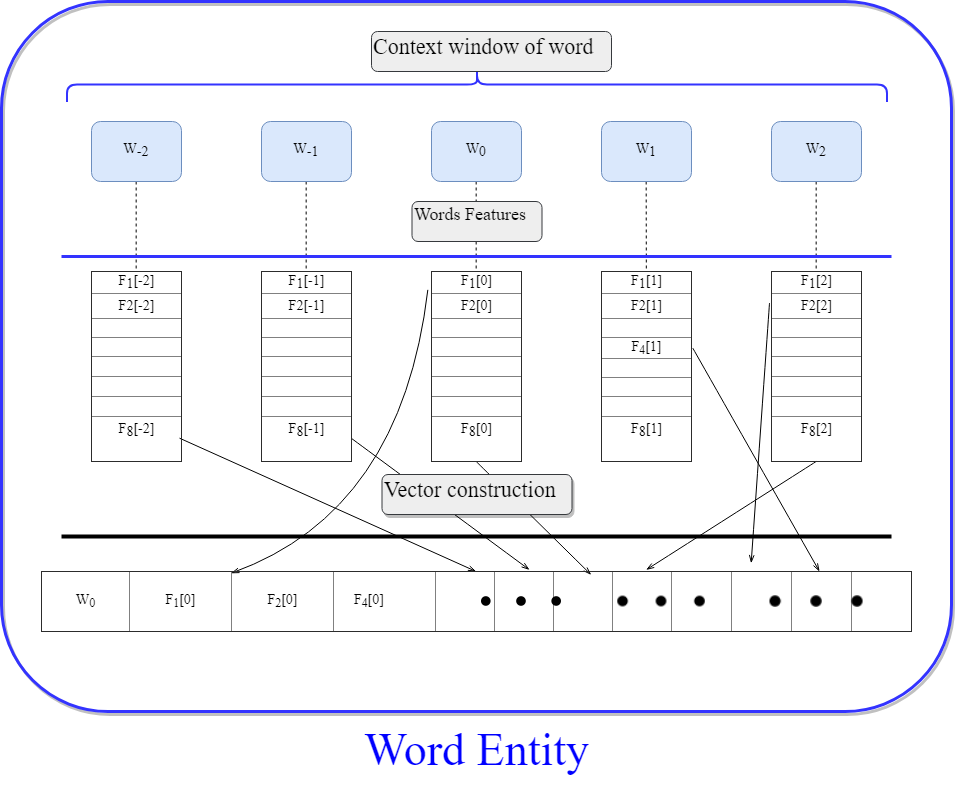
\includegraphics[width=0.8\linewidth]{wordEntity.png}
  \caption{Encapsulation of word features}\label{groupwordfeatures}
\endminipage\hfill
\minipage{0.5\textwidth}
    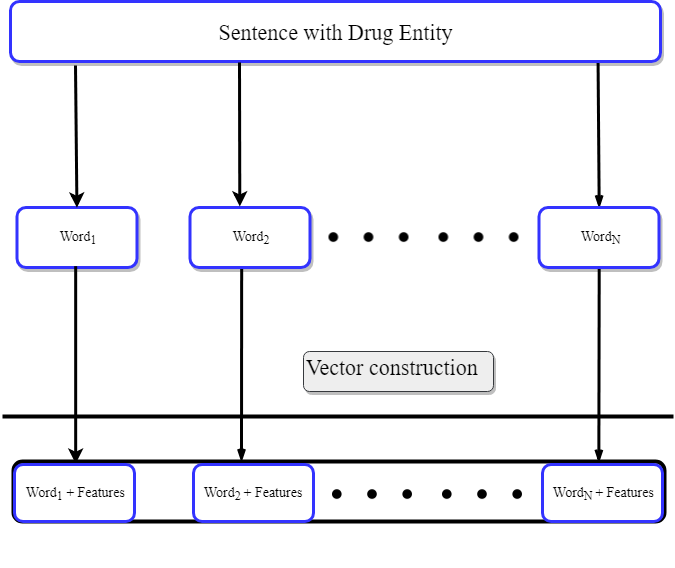
\includegraphics[scale=0.3]{CRF.png}\caption{DNR-CRF feature vector}\label{dnrcrf}
\endminipage
\end{figure}








